
\setbeamerfont{block title}{size=\scriptsize}
\setbeamerfont{block body}{size=\scriptsize}
\setbeamerfont{exampleblock title}{size=\scriptsize}
\setbeamerfont{exampleblock body}{size=\scriptsize}

\begin{frame}{Les systèmes de systèmes}
\centering 
%\begin{tabular}{cc}
%Dirigé & Consensuel \\
%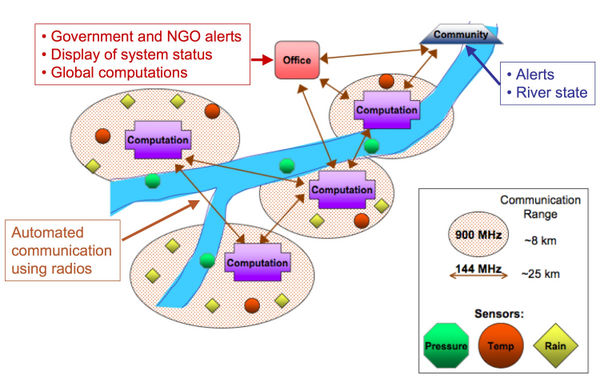
\includegraphics[width=3cm, height=2cm]{imgs/fms.jpeg} &
%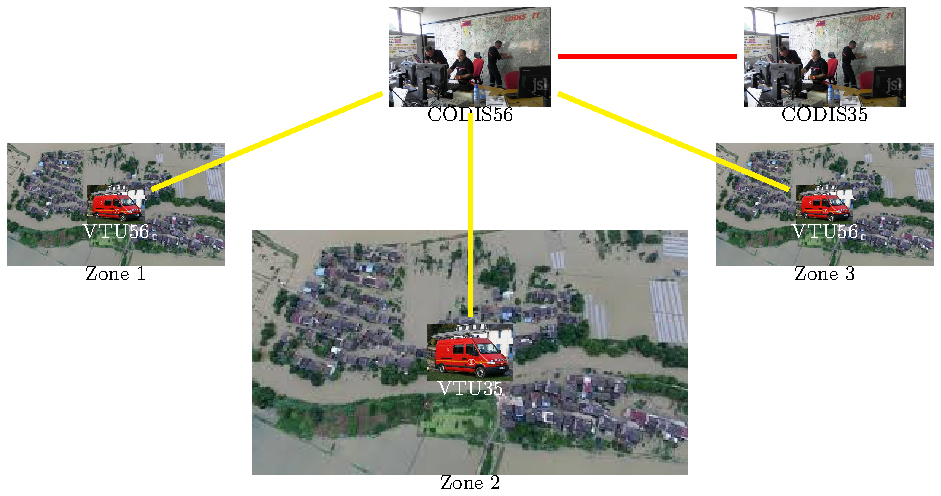
\includegraphics[width=3cm, height=2cm]{imgs/fig_overview_conf1.pdf}\\
%Surveillance d'inondation \vspace{0.2cm}& Service d'urgence\vspace{0.2cm}\\
%Collaboratif & Virtuel \\ 
%
\includegraphics[width=3cm, height=2cm]{imgs/internet.jpg} &
%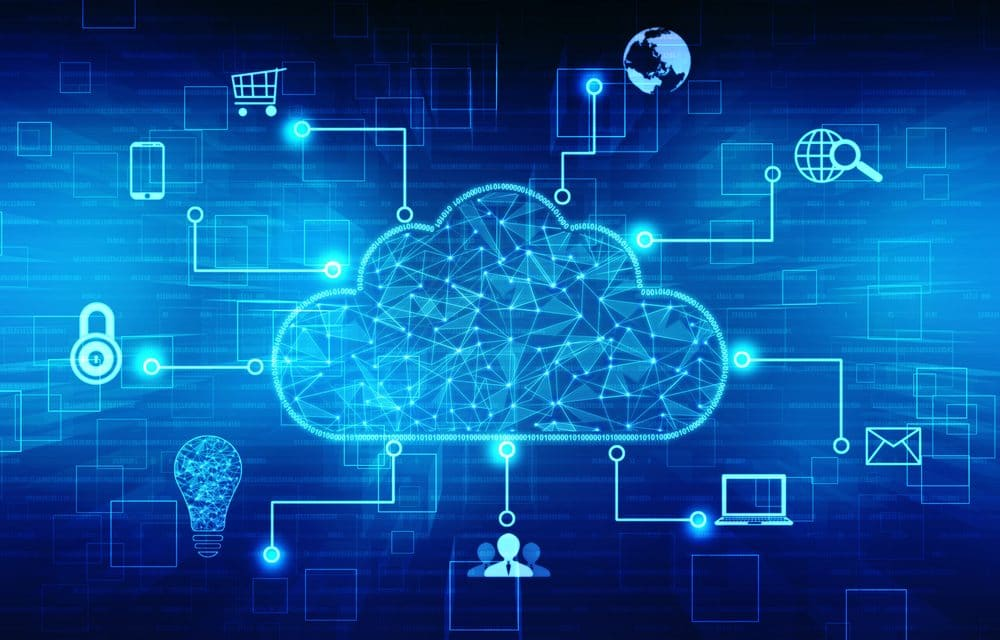
\includegraphics[width=3cm, height=2cm]{imgs/web.jpg}\\
%Internet & Web \\
%\end{tabular}
\begin{columns}
\begin{column}{0.4\textwidth}
\begin{block}{}
\begin{itemize}
\item  Ces systèmes participants (CSs) sont \textbf{géographiquement
distribués}, 
\item possèdent leur propre \textbf{indépendance
opérationnelle} et
\textbf{managériale}. 
\item L'intéraction de ces CSs produit un \textbf{comportement
émérgent}. 
\item Le SdS a un \textbf{développement évolutionnaire}.
\end{itemize} 
\end{block}
\end{column}
\begin{column}{0.5\textwidth}
\begin{figure}
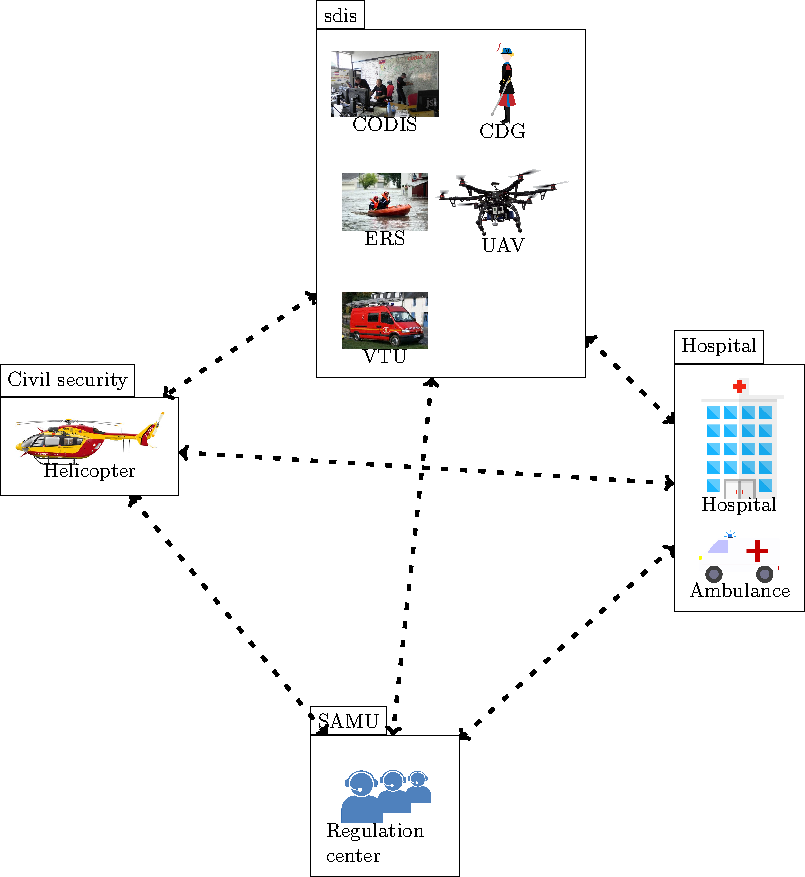
\includegraphics[height=\textwidth]{imgs/fig_sos_overview.pdf}
\caption{\underline{\textbf{Service de secours Français}}}
\end{figure}
\end{column}
\end{columns}
\end{frame}

\begin{frame}{Développement évolutionnaire}

\begin{textblock*}{4.5cm}(80mm,10mm)
\begin{block}{}
Le \textbf{développement évolutionnaire} est l'\textbf{évolution
constante} \\
des \textbf{fonctions} et \textbf{buts} du SdS.
\end{block}
\end{textblock*}

\begin{figure}
%\centering
\flushleft
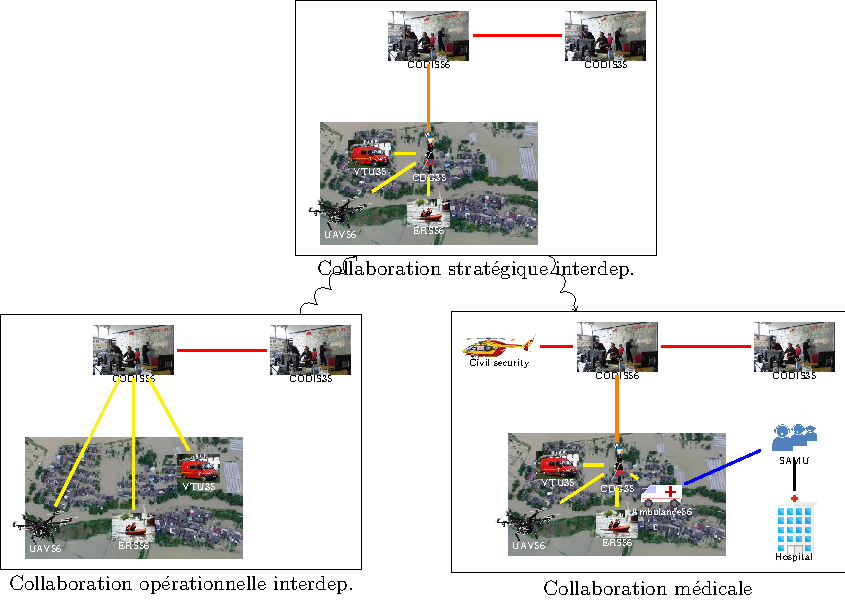
\includegraphics[width=9cm]{imgs/dev_evolutionnaire.pdf}
\end{figure}
\end{frame}


\begin{frame}{Problématique : variabilité des décisions reconfiguration dynamique}
\begin{block}{}
La \textbf{reconfiguration dynamique} est une phase du
developpement d'une système qui consiste à le modifier pendant qu’il est
utilisé. La reconfiguration peut-être corrective, fonctionnelle,  ou
non-fonctionnelle.
\end{block}
\begin{figure}
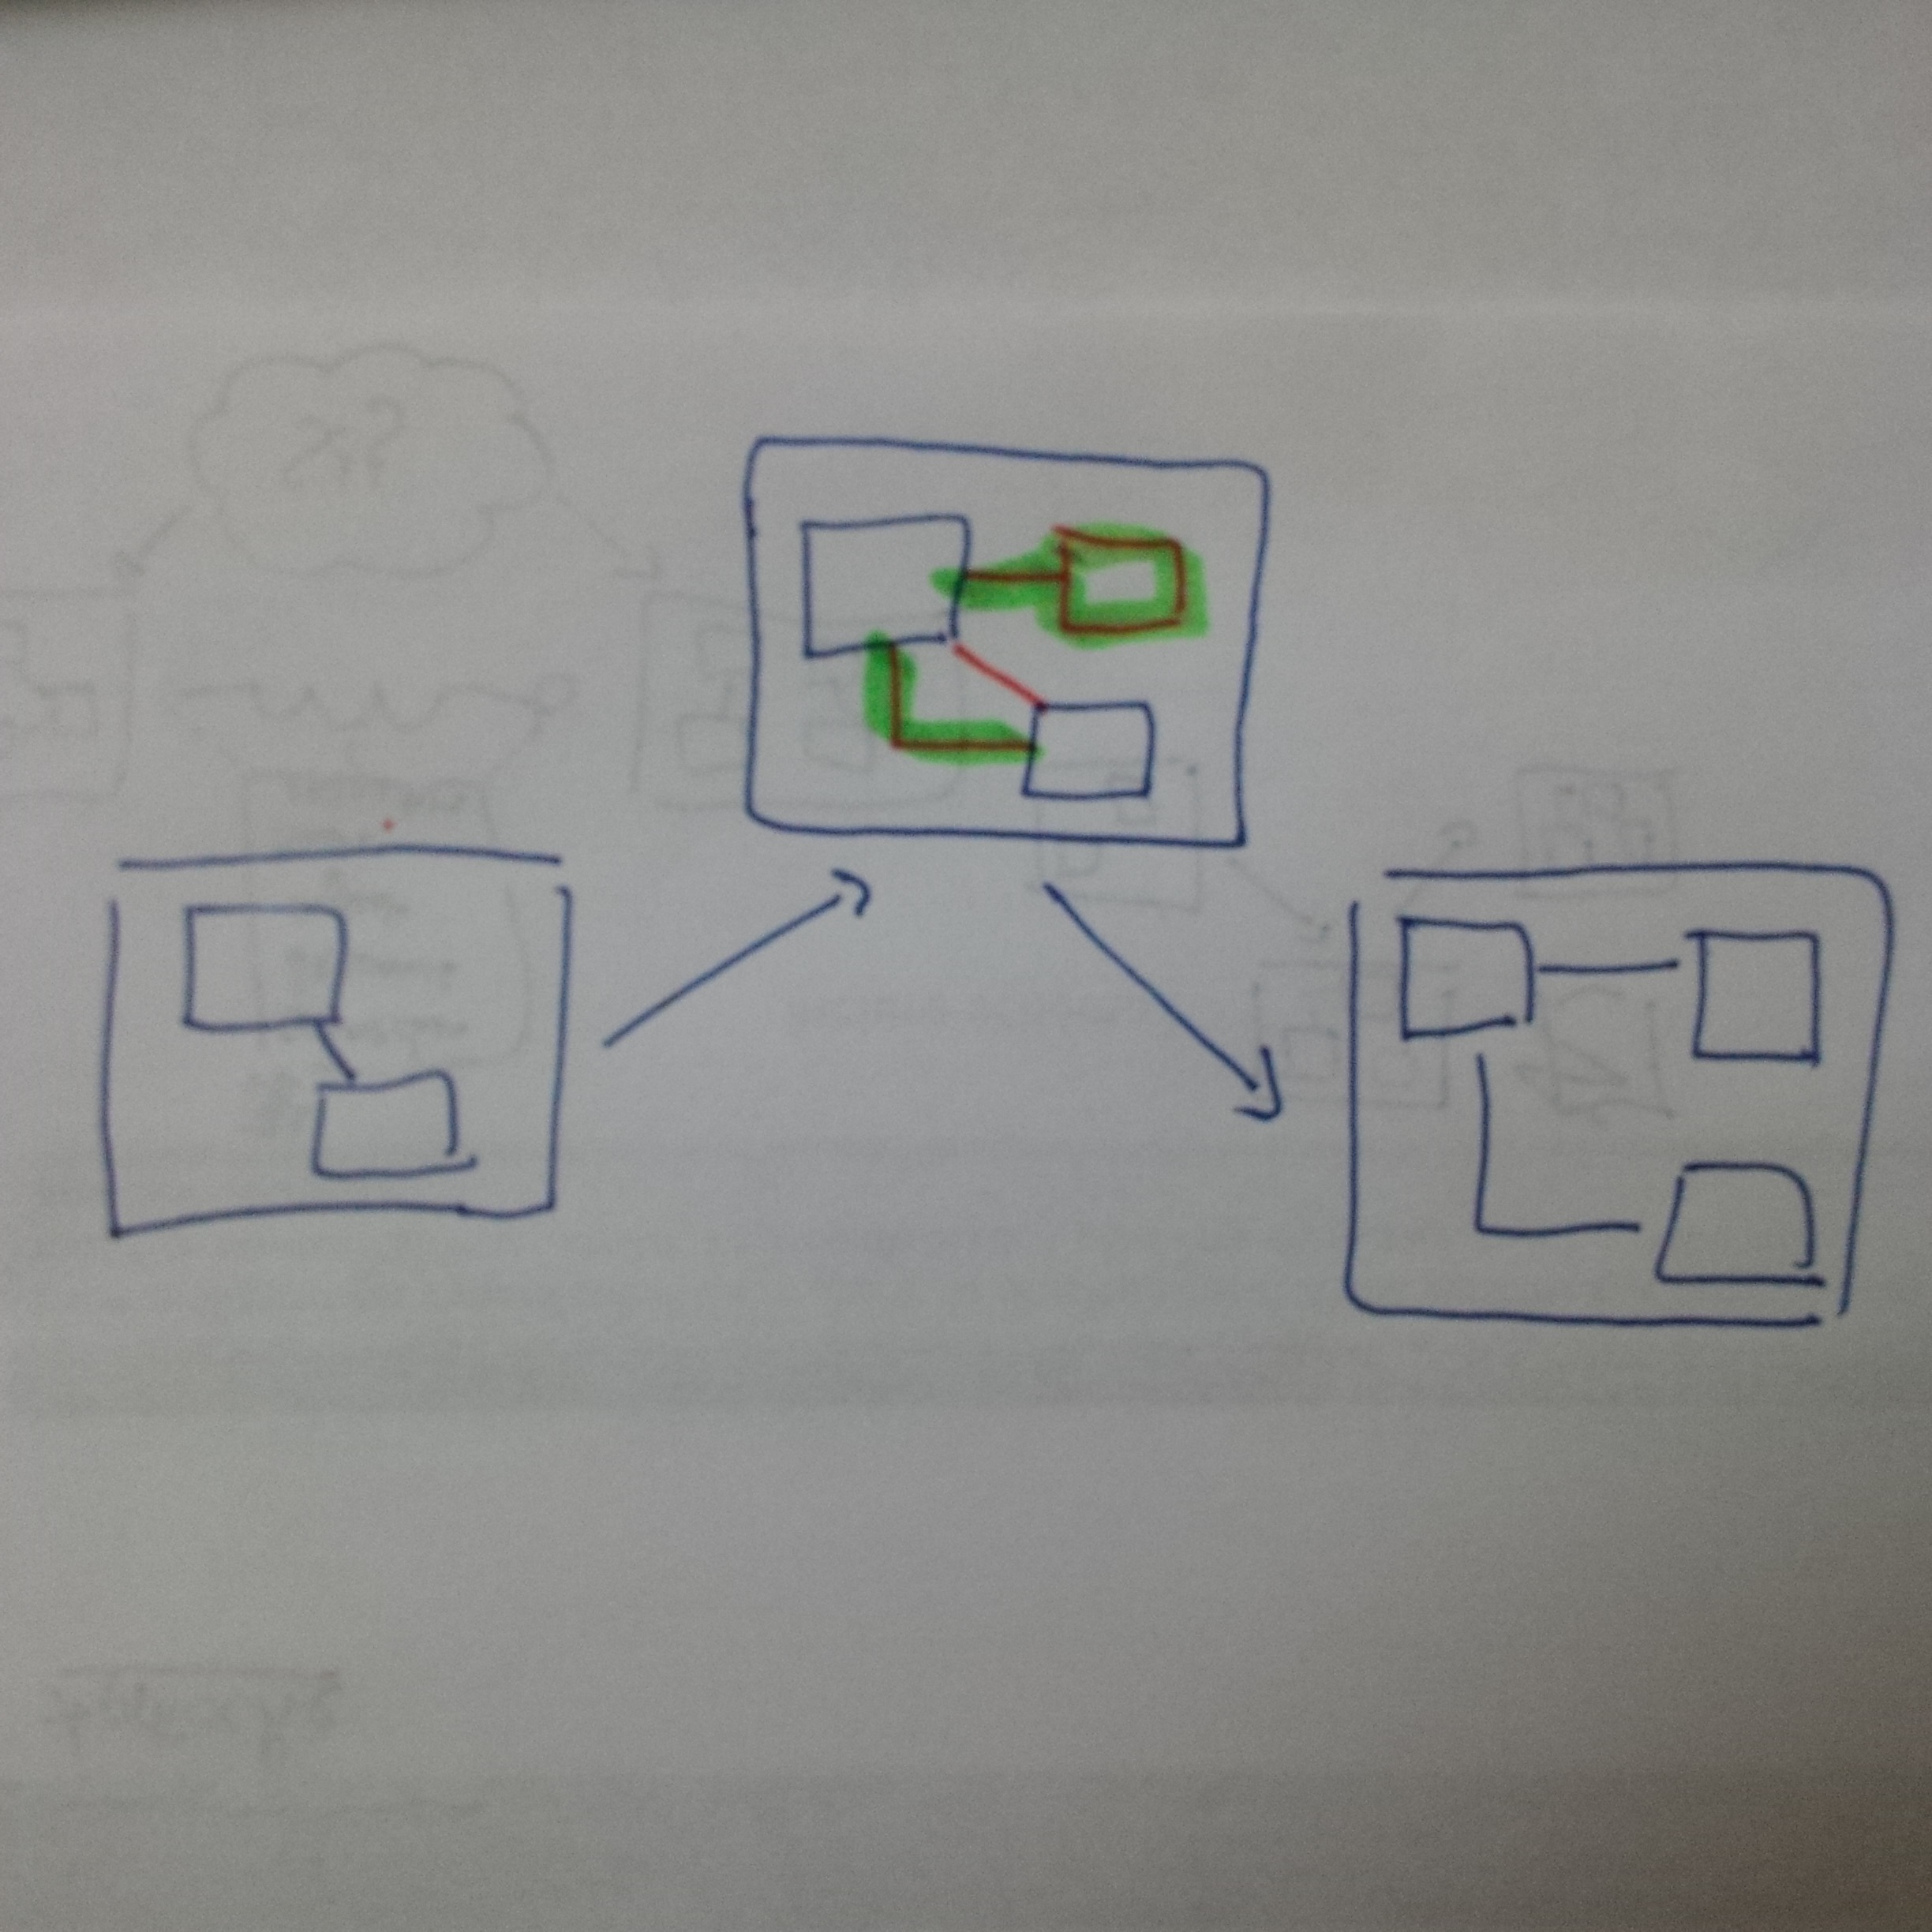
\includegraphics[height=6cm]{imgs/description_reconfiguration}
\end{figure}

Caractéristiques d'une reconfiguration pour SdS : 
\begin{itemize}
\item évolution du contexte de reconfiguration
\item opérations de reconfiguration hétérogène
\end{itemize}
\end{frame}
%
\begin{frame}{Solution : patron de reconfiguration et processus de
conception des reconfigurations}
\begin{figure}
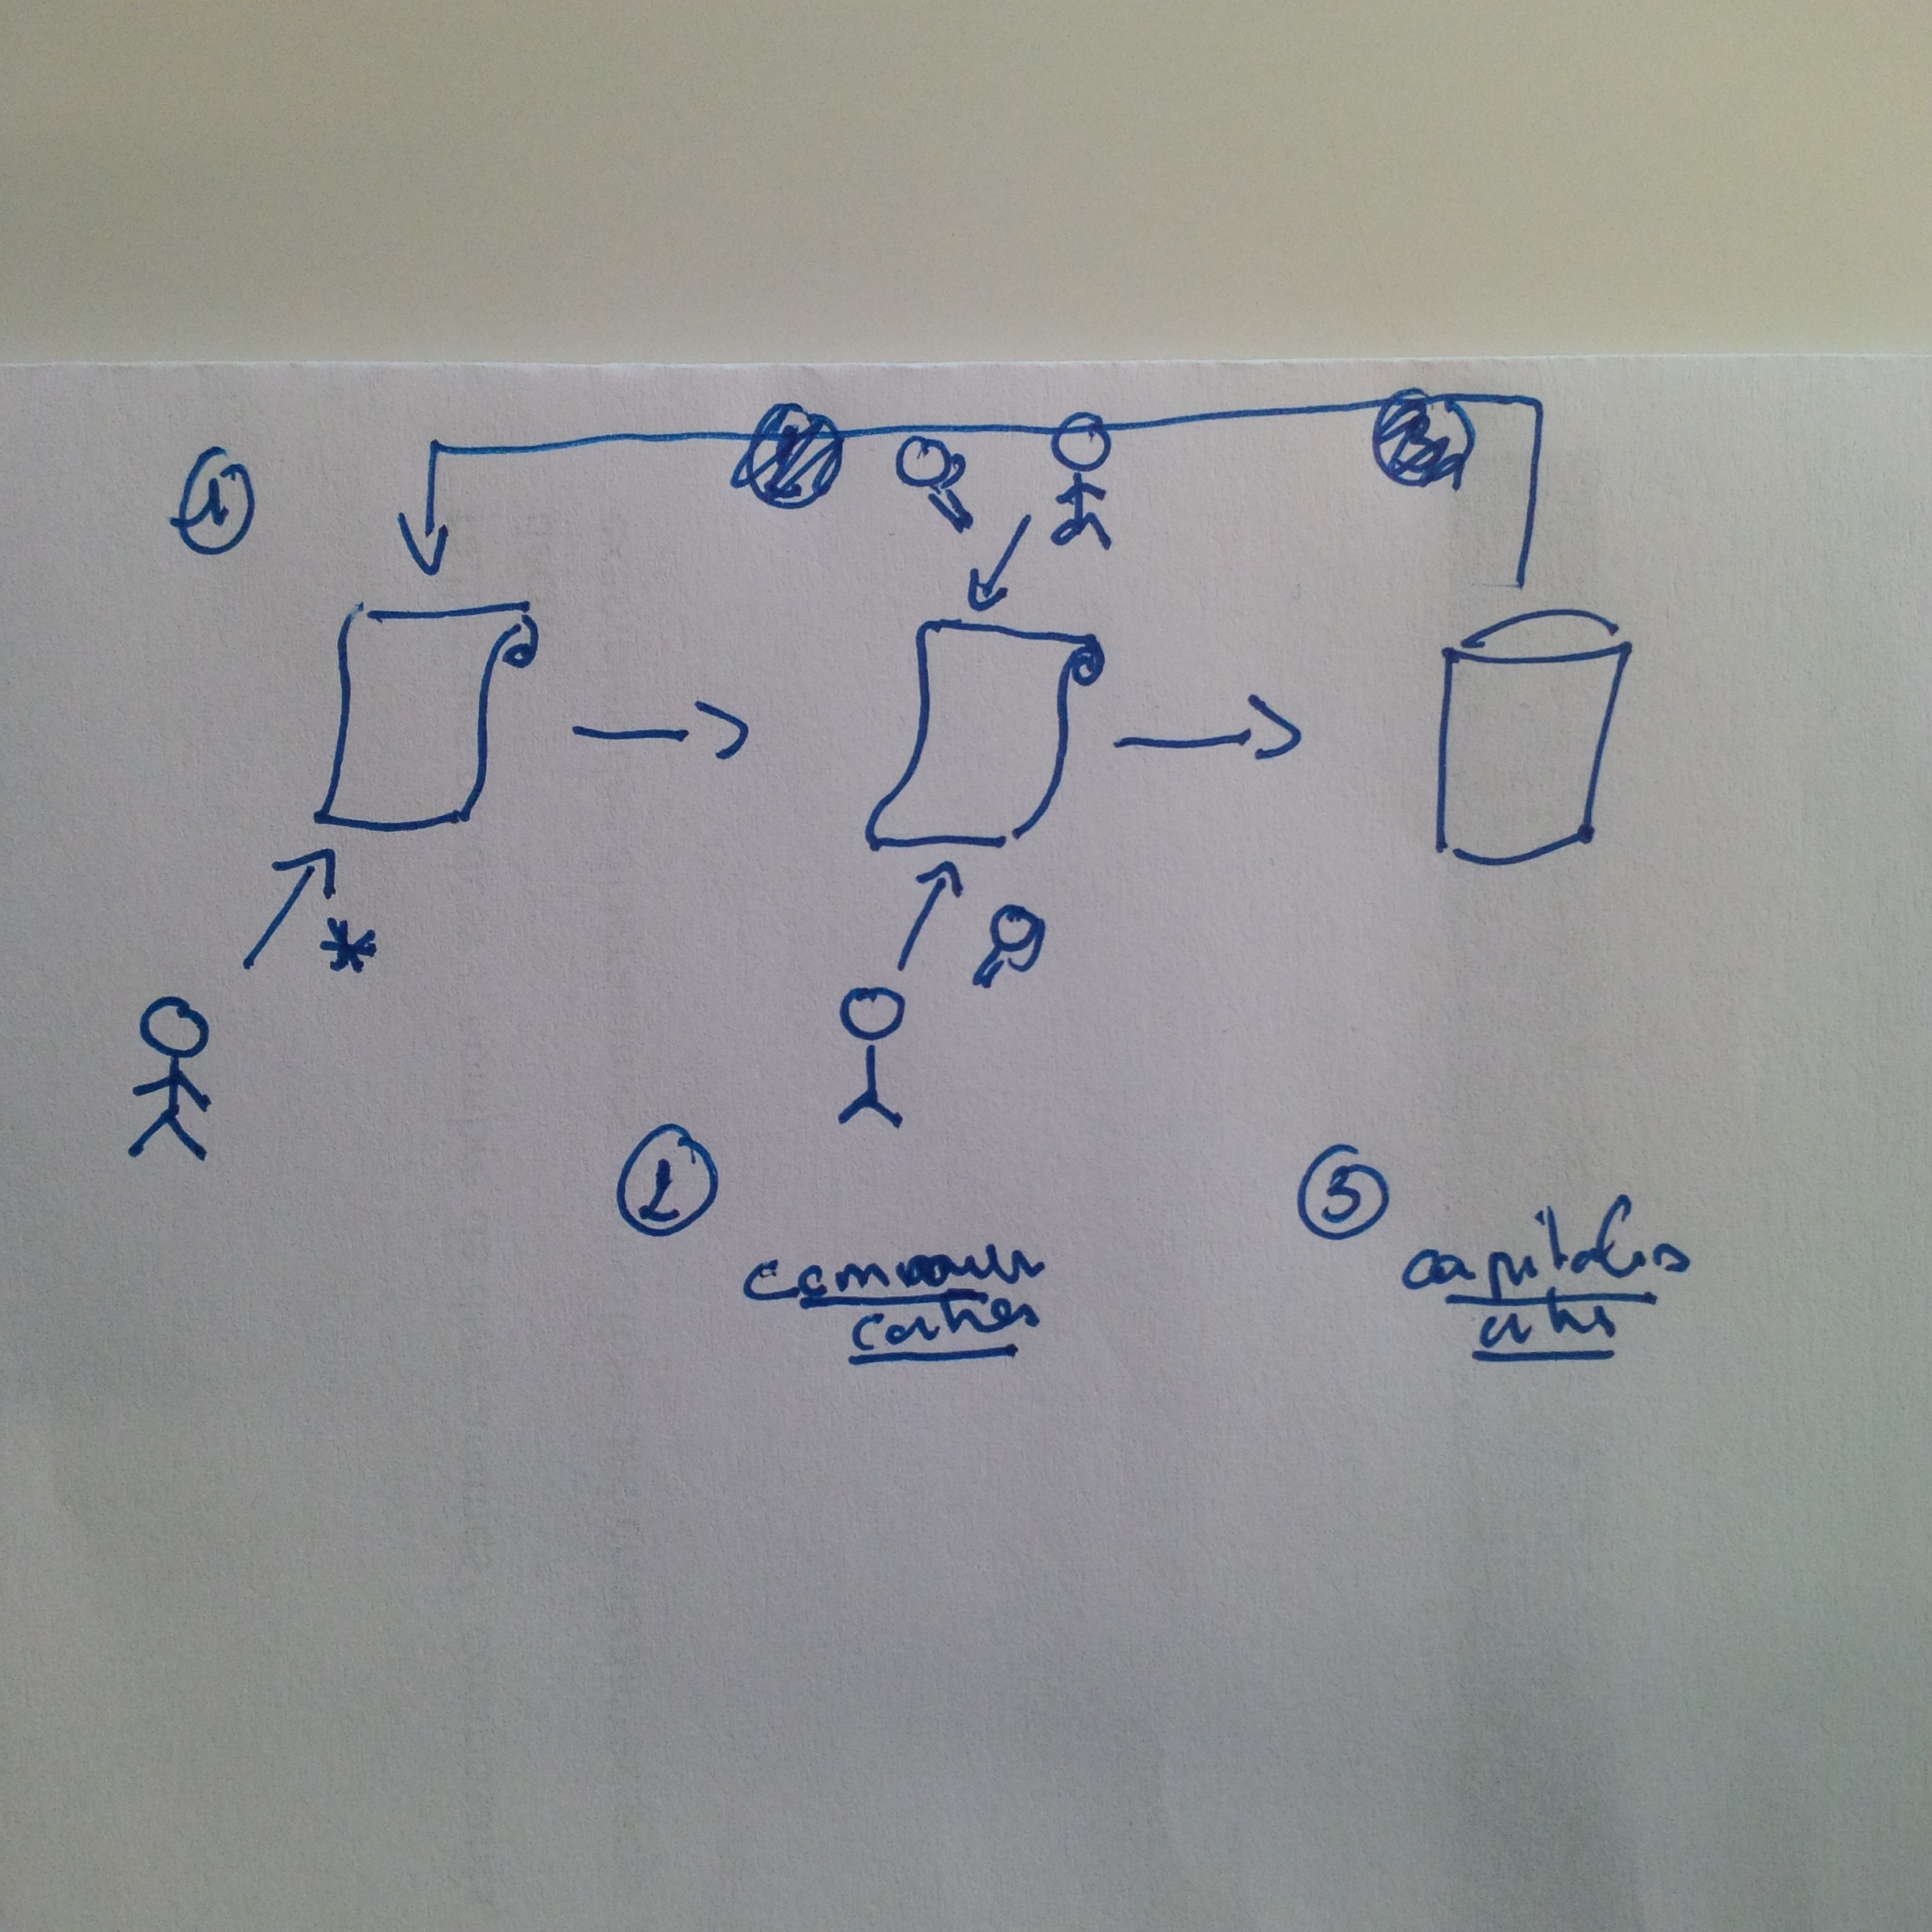
\includegraphics[width=10cm, height=3cm]{imgs/slide_application_patron}
\end{figure}
\begin{block}{}
Les \textbf{patrons de reconfiguration dynamique} documentent des solutions de
reconfiguration dynamique à des problèmes de conception récurrents.
\end{block}
%\begin{exampleblock}{}
%\begin{itemize}
%\item Programmation orientée objet : \textit{Design Patterns: Elements of
%Reusable Object-Oriented Software} 
%\item Architecture des systèmes distribués : \textit{Architecture,
%volume 4: A Pattern Language for Distributed Computing}
%\end{itemize}
%\end{exampleblock}
\end{frame}

%\begin{frame}{Problèmes rencontrés : modélisation de configuration}
%\begin{figure}
%\centering
%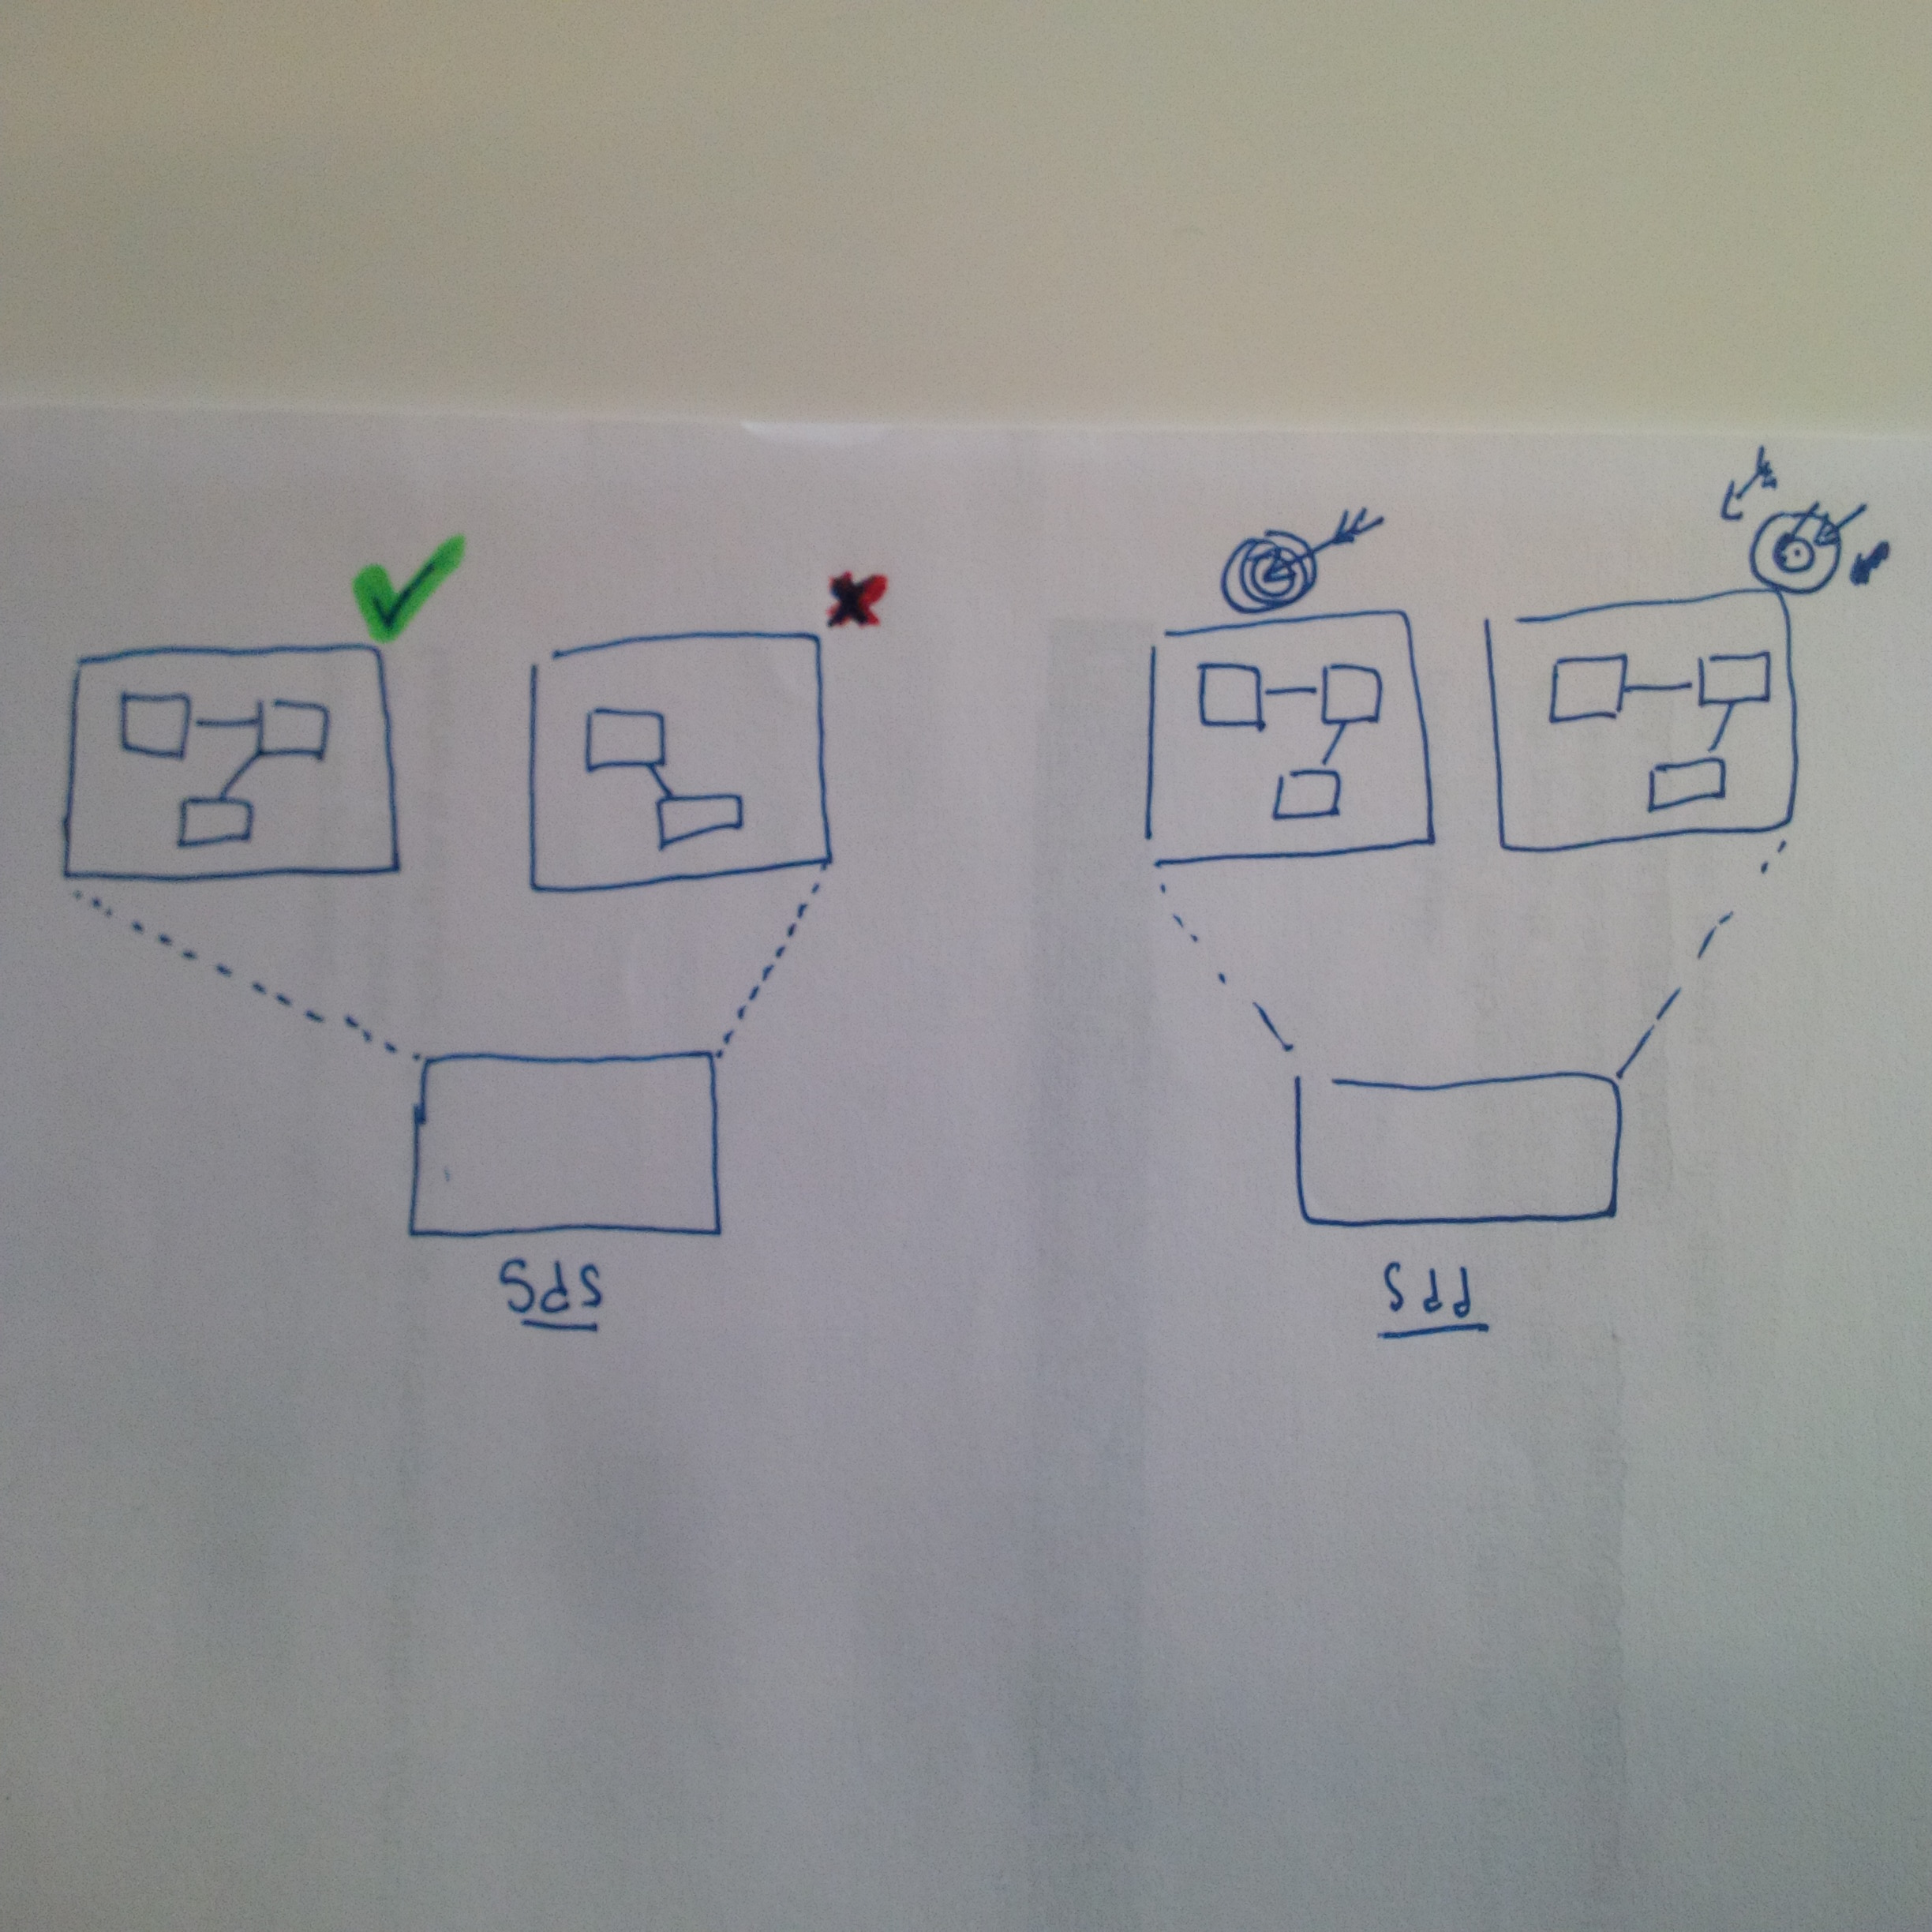
\includegraphics[width=10cm, height=4cm]{imgs/slide_probleme_modelisation.jpg}
%\end{figure} 
%\begin{definition}{}
%Un modèle est \textbf{exact} si il est
%factuel ou ne dévie pas trop du fait qu’il modélis
%\end{definition}
%\begin{definition}{}
%Un modèle est \textbf{précis} si il est suffisamment détaillé pour
%répondre au besoin de spécification, d'analyse ou de vérification.
%\end{definition}
%\end{frame}

%\begin{frame}{Problèmes recontrés : processus de reconfiguration}
%\begin{figure}
%\centering
%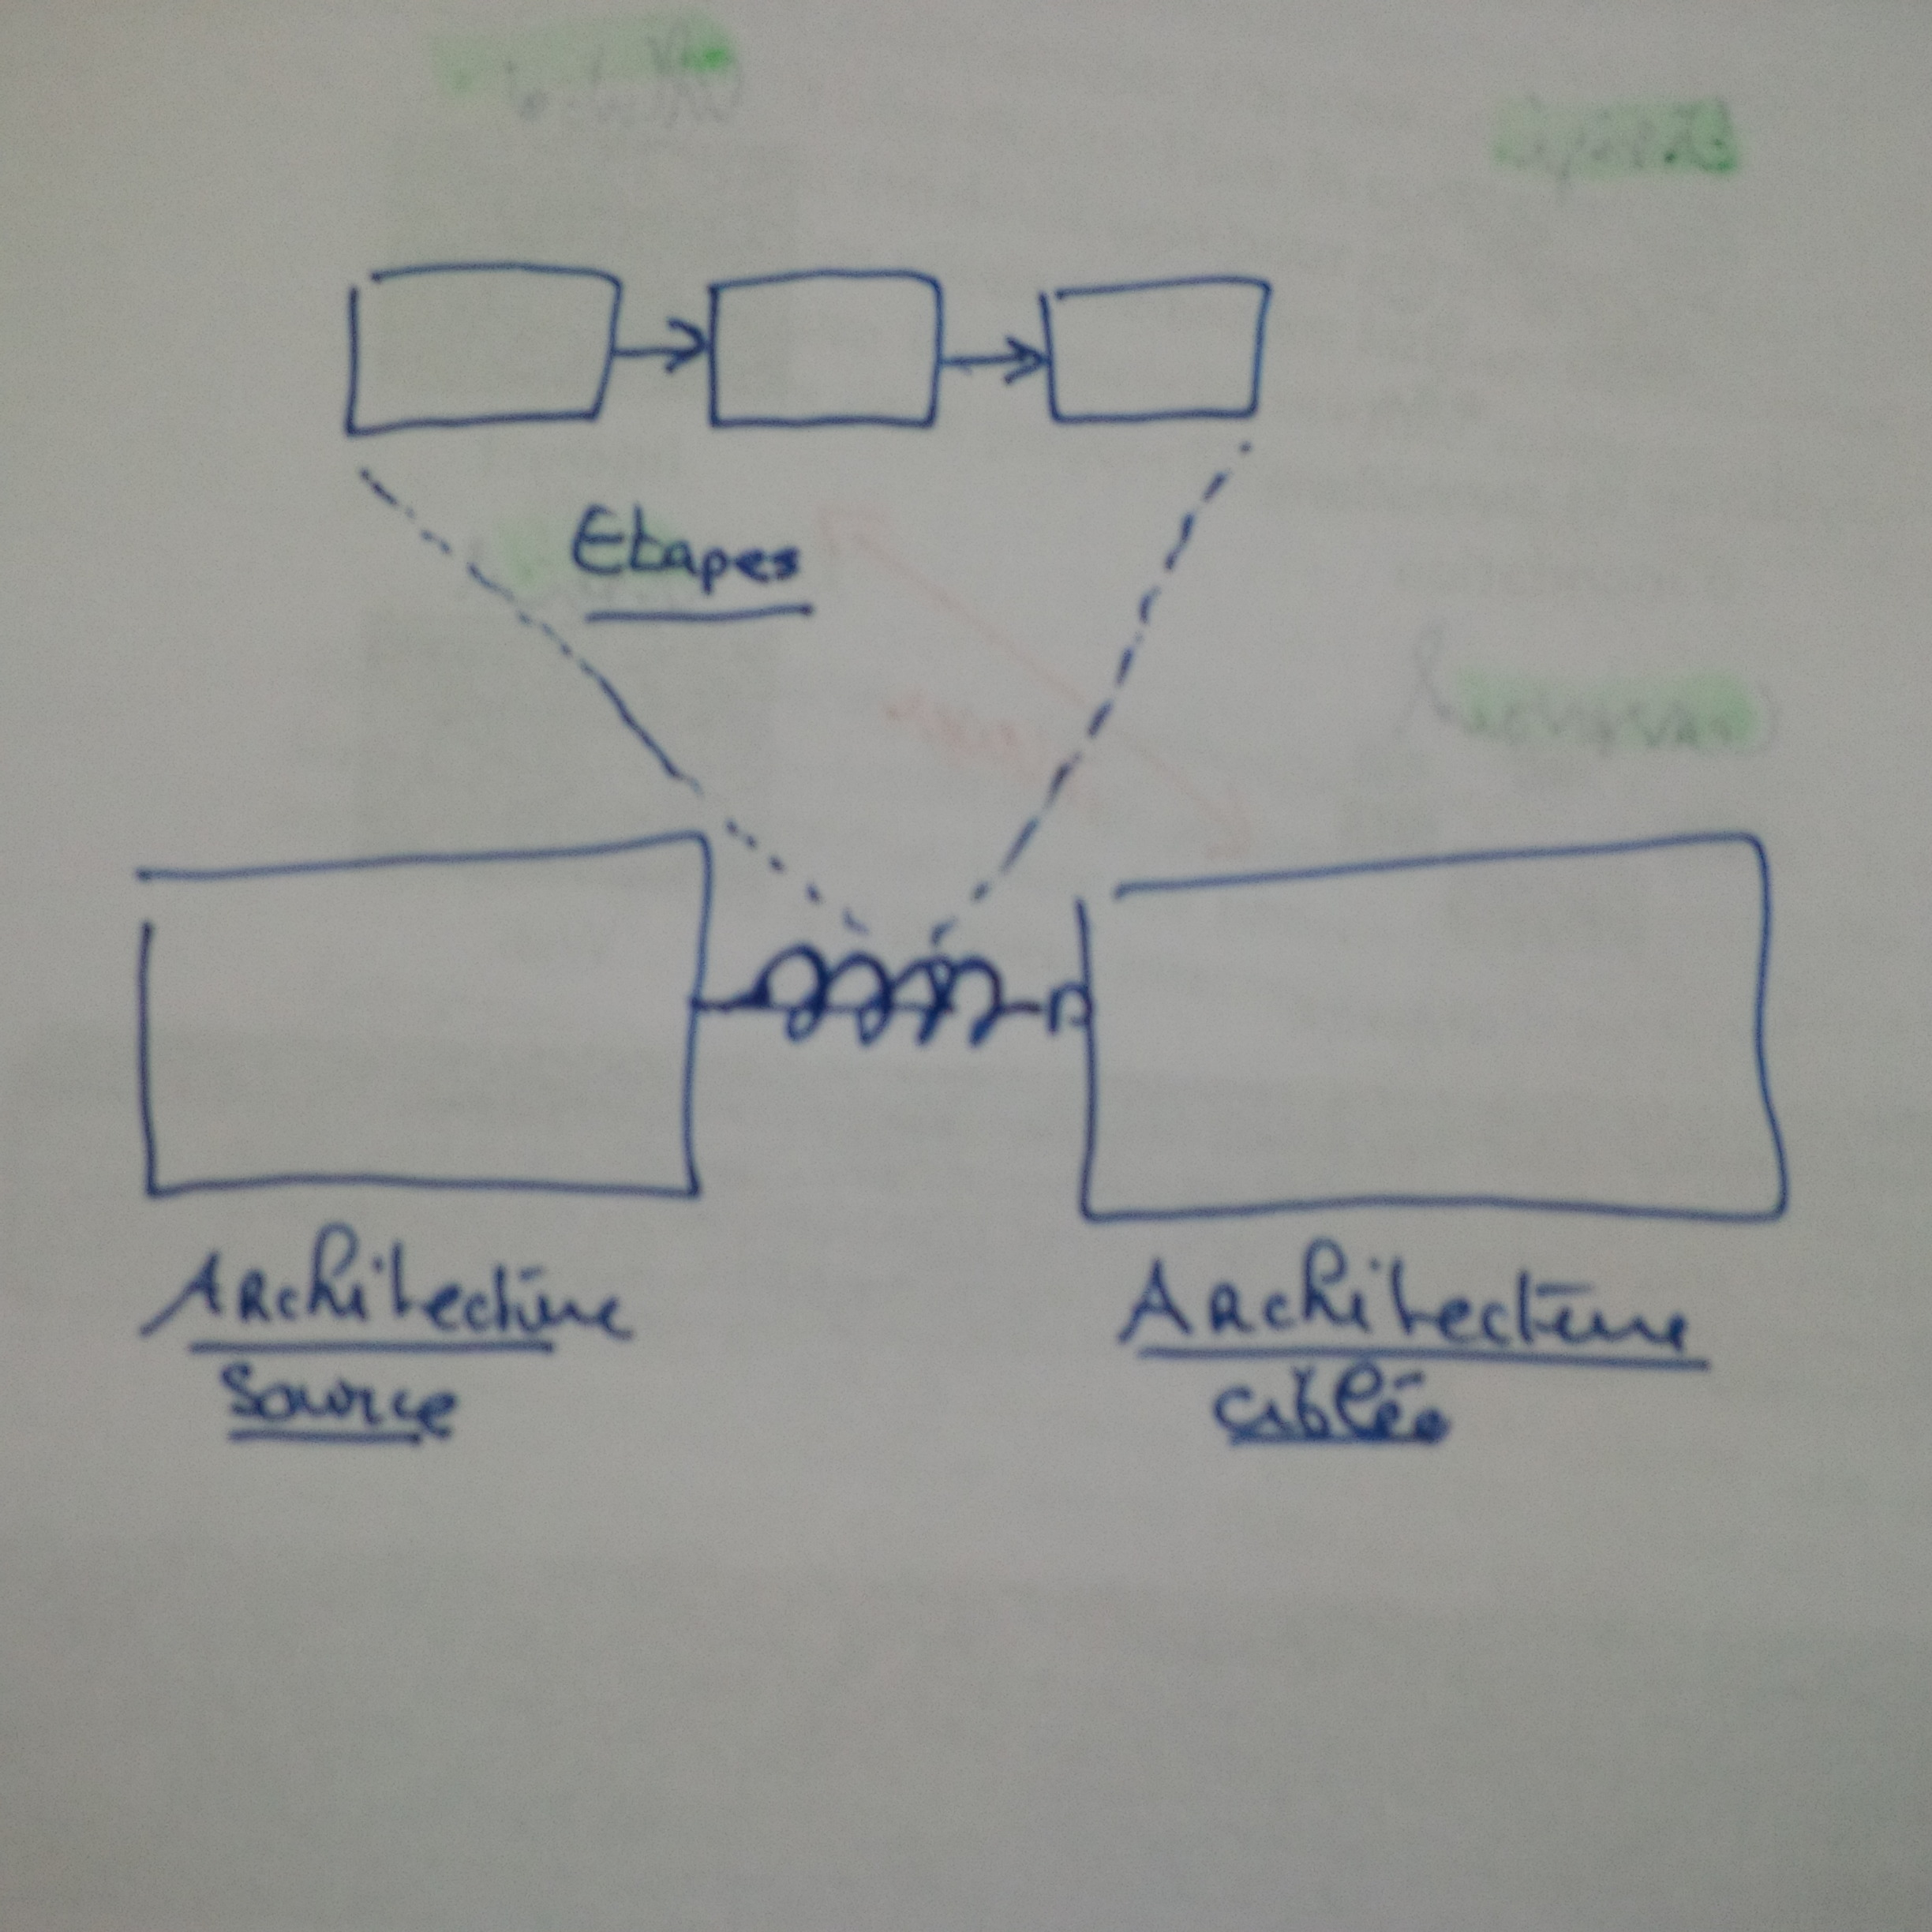
\includegraphics[width=\textwidth, height=0.6\textwidth]{imgs/slide_introduction_process.jpg}
%\end{figure}
%\end{frame}

\begin{frame}{Questions de recherche}
Comment l’architecte doit-il procéder pour faire évoluer un système de systèmes après son déploiement, dans le cadre du développement évolutionnaire ?\\
\begin{itemize}
    \item[Q1] Comment l’architecte modélise-t-il la configuration du système avec le niveau de précision et d’exactitude requis ?
    \item[Q2] Comment l’architecte peut-il documenter ses choix de conception d’une reconfiguration ?
    \item[Q3] Quel processus d’ingénierie l’architecte doit-il suivre pour concevoir la reconfiguration d’évolution du système de systèmes ?
\end{itemize}
\end{frame}

\begin{frame}{Plan de la soutenance}
\tableofcontents
\end{frame}

